Nick Vosseteig

2015-01-23

Building, Testing

\begin{tabular}{|p{5cm}|p{5cm}|}
 \hline
 Building&
This week I worked on fixing the gears on the spinner as well as fixing the intake device which was working incorrectly due to large amounts of friction. It went well. Everything we worked on this week now works and we made a lot of progress. 
 \\
 \hline
Testing&
We tested out the new cardboard prototype of the tube as well as the ramp which we moved back, the intake device and spinner. At first it wasn’t going well because the intake was not working as well as a wheel got disconnected, but as the week went on, we got everything working correctly.
 \\
 \hline
\end{tabular}

\section*{Testing}
We tested a lot this week and were able to successfully fill the entire 90 centimeter tube with balls in just a few minutes. We also fixed a lot of problems we noticed including the intake and the wheels not working correctly. 


\section*{Building}
	The first thing I did was replace the entire launcher/spinner because the gears were not going together well. There had been a lot of grinding from past testing and the competition. There was also some unnecessary friction. I rebuilt and replaced it to make sure all of it was in line and reduced the friction as much as possible. After that was completed, we realized that the intake was not working at all and a wheel had been disconnected. I replaced the wire which had a lot of strain on it to fix the wheel and then had to take apart the intake because a piece was grinding that we didn’t notice when we had built it the first time. Ben moved the linear slides to the side of the robot so that we can move the ramp to the very back of the robot to prevent the spinner from hitting it.

Here is a picture of where we moved the linear slides to:
\begin{center}
 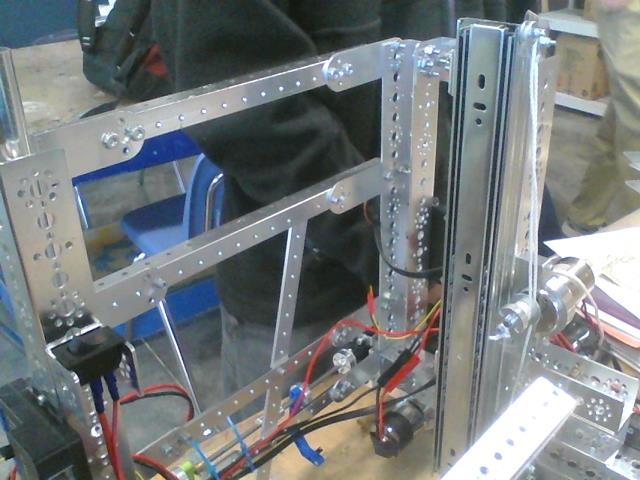
\includegraphics[width=215px]{./Entries/Images/slidesonside.jpg}
\end{center}
